\documentclass{templateNote}

\definecolor{Verde}{RGB}{170,239,31}
\definecolor{Morado}{RGB}{127,0,255}
\definecolor{Celeste}{RGB}{0,191,255}
\definecolor{Salmon}{RGB}{255,0,157}
\definecolor{RosaSuave}{RGB}{255,182,193}
\definecolor{Melocoton}{RGB}{255,218,185}
\definecolor{Gris}{RGB}{192,192,192}
\definecolor{Turquesa}{RGB}{64,224,208}
\definecolor{Menta}{RGB}{152,251,152}
\definecolor{AmarilloVainilla}{RGB}{255,255,153}

\newcommand{\newparagraph}{\par\vspace{\baselineskip}\noindent}
\newcommand{\hlcolor}[2]{{\sethlcolor{#1}\hl{#2}}}

\begin{document}

\imagenlogoU{img/LogoElNube.png}
\linklogoU{https://github.com/MarceloPazPezo}
\linkQRDoc{https://github.com/MarceloPazPezo/MyRepo/blob/main/Icinf/Semestre\%207/Investigaci\%C3\%B3n\%20de\%20Operaciones/Certamen-2/Certamen-2.pdf}
\titulo{Certamen 2}
\asignatura{Investigación de Operaciones}
\autor{
Marcelo Paz
}
\vDoc{1.0.0}
\tipoDoc{Apunte}

% Metadatos del PDF
\title{[\asignatura]-\titulo}
\author{
    \autor
}
\portada
\margenes % Crear márgenes

\section{Lineas de Espera}
Es un modelo matem\'atico que permite analizar el comportamiento de un sistema de espera.
\begin{itemize}
    \item \textbf{Objetivo:} Minimizar el tiempo de espera de los clientes y el costo de atenci\'on.
    
    \item \textbf{Aplicaciones:} Aeropuertos, hospitales, bancos, supermercados, etc.
\end{itemize}
\begin{figure}[H]
    \centering
    
\includegraphics[width=\textwidth]{diagram/LineaDeEspera.png}
\end{figure}
\newparagraph

\subsection*{Cantidad de Clientes en el Sistema}
\begin{figure}[H]
    \centering
    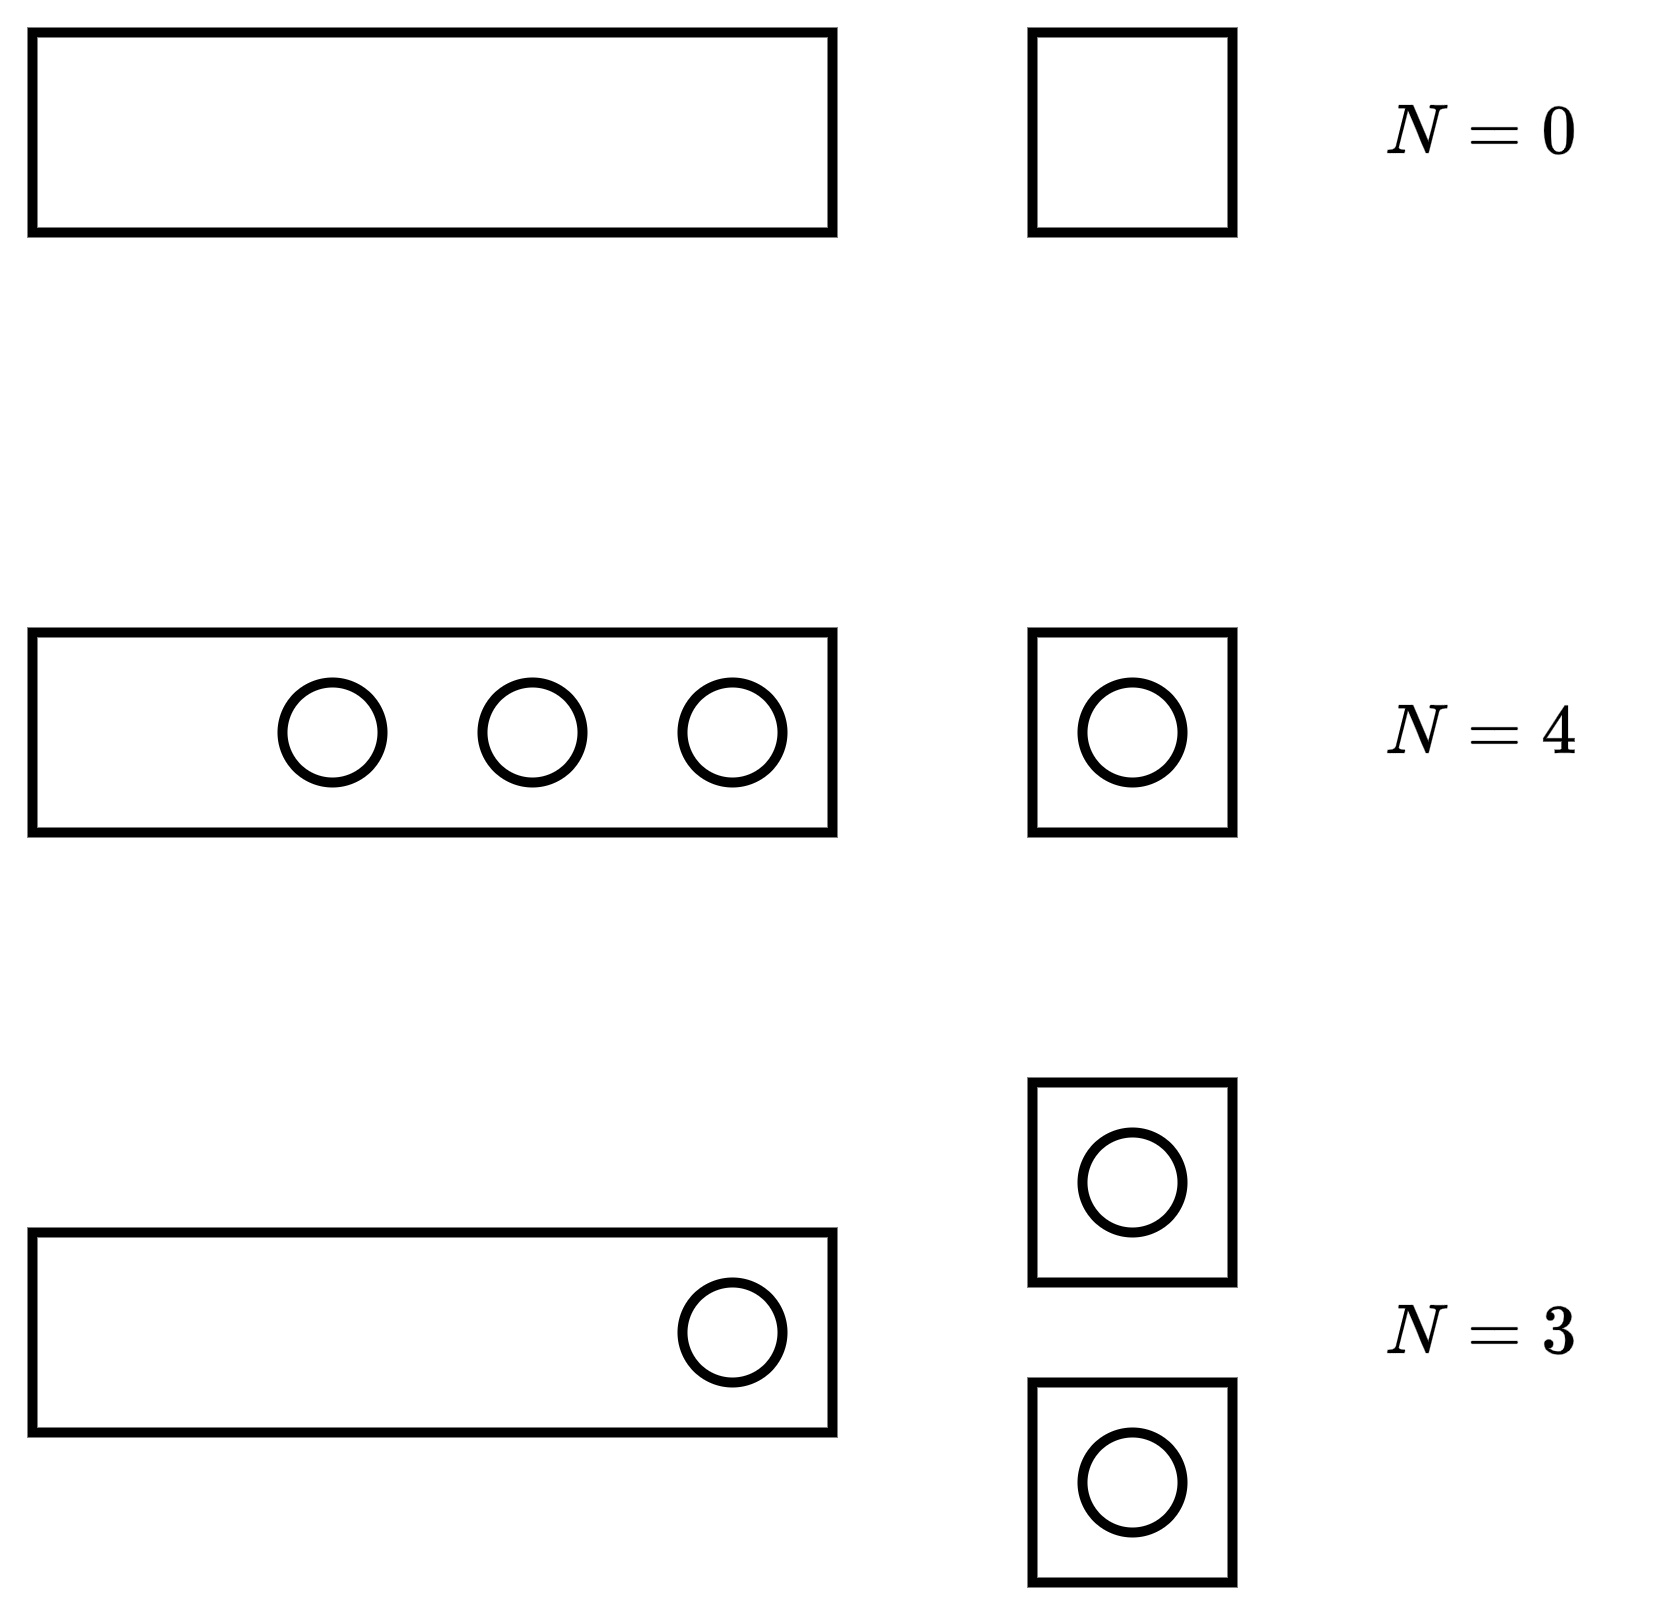
\includegraphics[width=0.5\textwidth]{diagram/Nclientes.png}
\end{figure}

\newpage
\subsection{\'Unico Servidor (M/M/1)}
\noindent
\textbf{Notaci\'on de Kendall:} \hlcolor{Menta}{M}/\hlcolor{Morado!50}{M}/\hlcolor{Turquesa}{1} se refiere a un sistema de colas con una \hlcolor{Menta}{tasa de llegada de clientes $\lambda$}, una \hlcolor{Morado!50}{tasa de servicio $\mu$} y \hlcolor{Turquesa}{1 servidor}.
\newparagraph
El sistema de espera se caracteriza por:
\begin{itemize}
    \item Los tiempos de llegadas y los tiempos de servicio se distribuyen de manera exponencial.
    
    \item Un \'unico servidor.
    
    \item Tiene el formato FIFO (First In First Out).
    
    \item El tama\~no de la poblaci\'on de entrada es infinito, es decir, el n\'umero de clientes en el sistema no afecta a la tasa de llegada.
    
    \item La tasa de servicio no depende del n\'umero de clientes en el sistema.
    
    \item Para que el sistema sea estable, se debe cumplir la \textbf{Condici\'on de regimen}.
    \begin{equation*}
        \rho < 1
    \end{equation*}
    Esta condici\'on tiene el objetivo de que la tasa de llegada sea menor a la tasa de servicio, pues como la capacidad del sistema es infinita, si la tasa de llegada es mayor a la tasa de servicio, el sistema se saturar\'a.
\end{itemize}
\begin{center}
    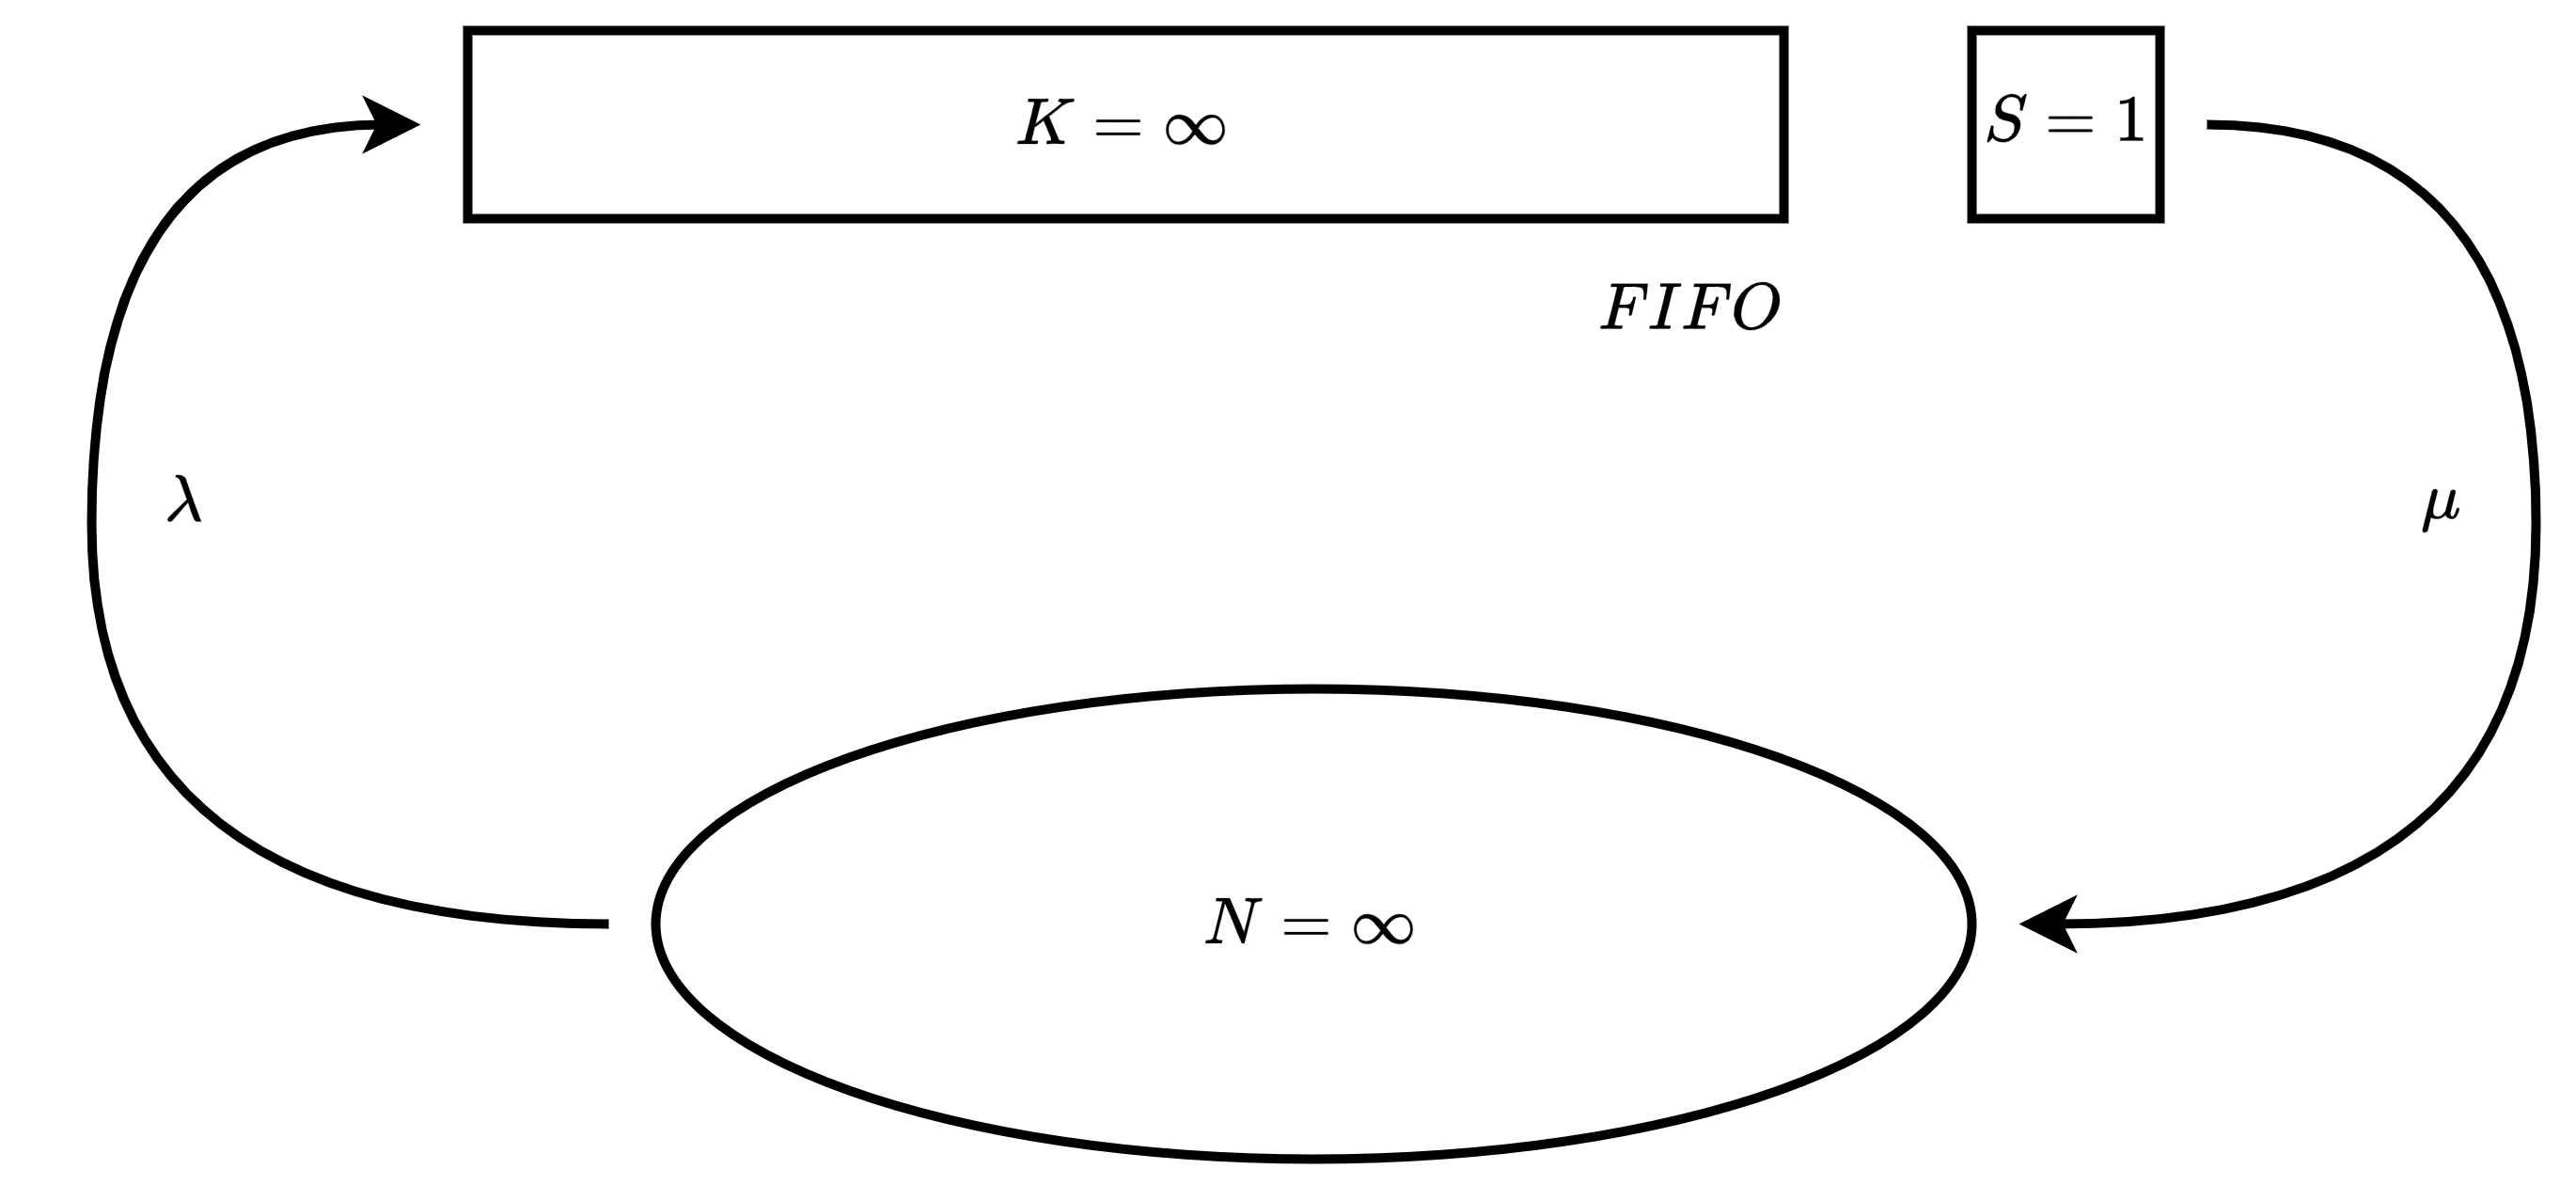
\includegraphics[width=0.8\textwidth]{diagram/mm1.png}
\end{center}

Donde:
\begin{itemize}
    \item $K$ : Capacidad del sistema.
    
    \item $S$ : Número de servidores en paralelo.
    
    \item $\mu$ : Tasa de servicio medidas (Clientes / Unidad de tiempo).
    
    \item $N$ : Número de clientes en el sistema.
    
    \item $\lambda$ : Tasa de llegada de clientes (Clientes / Unidad de tiempo)
\end{itemize}

\newpage
\subsubsection{Indicadores (Performance)}
\textbf{IMPORTANTE:} Para los cálculos, se debe considerar la misma unidad de tiempo.
\begin{itemize}
    \item $L$ : Cantidad promedio de clientes en el sistema.
    \begin{equation*}
        L = \frac{\lambda}{\mu - \lambda}
    \end{equation*}

    \item $L_q$ : Cantidad promedio de clientes en la cola.
    \begin{equation*}
        L_q = \frac{\lambda^2}{\mu(\mu - \lambda)}
    \end{equation*}

    \item $W$ : Tiempo promedio de un cliente en el sistema.
    \begin{equation*}
        W = \frac{L}{\lambda} = \frac{1}{\mu - \lambda}
    \end{equation*}

    \item $W_q$ : Tiempo promedio de un cliente en la cola.
    \begin{equation*}
        W_q = \frac{L_q}{\lambda} = \frac{\lambda}{\mu(\mu - \lambda)}
    \end{equation*}
\end{itemize}

\subsubsection{Probabilidades}
Sea $n$ : Cantidad de clientes en el sistema. ($n=1,2,...$)
Entonces:
\begin{itemize}
    \item $\rho$ : Factor de utilizaci\'on / Factor de carga / Intensidad tr\'afico.
    \begin{equation*}
        \rho = \frac{\lambda}{\mu} = 1 - P_0
    \end{equation*}
    \item $P_0$ : Probabilidad de que ning\'un cliente se encuentre en el sistema.
    \begin{equation*}
        P_0 = 1 - \frac{\lambda}{\mu}
    \end{equation*}
    
    \item $P_n$ : Probabilidad de que haya $n$ clientes en el sistema.
    \begin{equation*}
        P_n = \rho^n \cdot P_0 \qquad \text{Condici\'on de regimen} \quad \rho < 1
    \end{equation*}

    \item $P(W_q > t)$ : Probabilidad que un cliente este en la cola a lo menos $t$ unidades de tiempo.
    \begin{equation*}
        P(W_q > t) = \rho e^{-\mu(1 - e)\cdot t}
    \end{equation*}

    \item $P(W > t)$ : Probabilidad que un cliente permanezca en el sistema, a lo menos $t$ unidades de tiempo.
    \begin{equation*}
        P(W > t) = e^{-\mu(1 - e)\cdot t}
    \end{equation*}
\end{itemize}

\newpage
\subsubsection{Problema 1:}
En el mostrador de facturaci\'on de una aerol\'inea llega un promedio de 45 clientes por hora, cuando su capacidad media es de 60 clientes por hora.
Si un cliente espera una media de 3 minutos en la cola, se pide:
\begin{tcolorbox}[
    colframe=Celeste!100, % Color del borde
    colback=Celeste!20,       % Color del fondo
    coltitle=white!100, % Color del título
    title=\textbf{Datos}, % Título de la caja
]
        $\lambda = 45 \text{ clientes/hora}$ \\
        $\mu = 60 \text{ clientes/hora}$ \\
        $W_q = 3 \text{ minutos}$ \\
        $\rho = \frac{\lambda}{\mu} = \frac{45}{60} = \frac{3}{4} < 1 \quad \text{Condici\'on de regimen}$
\end{tcolorbox}
\begin{enumerate}
    \renewcommand{\labelenumi}{\alph{enumi})}
    \item Tiempo medio que un cliente pasa en la facturaci\'on.
    \begin{align*}
        W &= \frac{L}{\lambda} = \frac{1}{\mu - \lambda} = \frac{1}{60 - 45} = \frac{1}{15} \cdot 60 \text{ minutos} \\
        &= 4 \text{ minutos} 
    \end{align*}

    \item N\'umero medio de clientes en la cola.
    \begin{align*}
        L_q &= \frac{\lambda^2}{\mu (\mu - \lambda)} = \frac{45^2}{60(60-45)} = \frac{2025}{900} \\
        &= 2,25 \text{ clientes}
    \end{align*}
    \item N\'umero medio de clientes en el sistema en un momento dado.
    \begin{align*}
        L &= \frac{45}{(60-45)} = 3 \qquad \text{(Inventado)}
    \end{align*}

    \item Probabilidad de que el sistema est\'e vac\'io.
    \begin{align*}
        P_0 &= 1 - \frac{\lambda}{\mu} \\
        &= 1 - \frac{45}{60} = \frac{4-3}{4} \\
        &= \frac{1}{4} = 0,25 \\
        &= 25\%
    \end{align*}

    \item Probabilidad de que haya m\'as de 3 clientes:
    \begin{align*}
        P(n > 3) &= 1 - P(n \leq 3) = 1 - (P_0 + P_1 + P_2 + P_3) \\
        &= 1 - (0.25 + 0.1875 + 0.14 + 0.1054) \\
        &= 1 - 0.6829 = 0.3171 \\
        &= 31.71\%
    \end{align*}
\end{enumerate}

\newpage
\subsubsection{Problema 2:}
En un restaurante de carretera llega una media de 90 personas a la hora, cuando tiene disponibilidad de dar servicio a 120 clientes por hora. Sabiendo que los clientes esperan una media de 2 minutos en la cola, se pide:
\begin{tcolorbox}[
    colframe=Celeste!100, % Color del borde
    colback=Celeste!20,       % Color del fondo
    coltitle=white!100, % Color del título
    title=\textbf{Datos}, % Título de la caja
]
    $\lambda = 90$ \\
    $\mu = 120$ \\
    $W_q = 2 \text{ minutos}$ \\
    $\rho = \frac{90}{120} = \frac{3}{4} < 1 \qquad \text{Condici\'on de regimen}$
\end{tcolorbox}
\begin{enumerate}
    \renewcommand{\labelenumi}{\alph{enumi})}
    \item Probabilidad que el sistema se encuentre sin ocupar.
    \begin{align*}
        P_0 &= 1 - \rho = 1 - \frac{3}{4} = 0.25\\
        &= 25\%
    \end{align*}
    
    \item Probabilidad que un cliente tenga que esperar al encontrarse el sistema ocupado.
    \begin{align*}
        P(n > 1) &= 1 - P(n \leq 1) = 1 - (P_0 + P_1) \\
        &= 1 - (0.25 + (\frac{3}{4} \cdot 0.25)) = 1 - (0.25 + 0.1875) = 1 - 0.4375 = 0.5625 \\
        &= 56.25\%
    \end{align*}
    
    \item N\'umero medio de clientes en la cola.
    
    \item Probabilidad de que hay 4 clientes en la cola.
    \begin{align*}
        P_4 &= \rho^4 \cdot P_0 =\left(\frac{3}{4}\right)^2 \cdot 0.25 = 0.5625 \cdot 0.25 = 0.140625\\
        &= 14.0625\%
    \end{align*}
\end{enumerate}

\newpage
\subsection{Multiples Servidores en Paralelo (M/M/S)}
\noindent
\textbf{Notaci\'on de Kendall:} \hlcolor{Menta}{M}/\hlcolor{Morado!50}{M}/\hlcolor{Turquesa}{S} se refiere a un sistema de colas con una \hlcolor{Menta}{tasa de llegada de clientes $\lambda$}, una \hlcolor{Morado!50}{tasa de servicio $\mu$} y una cantidad \hlcolor{Turquesa}{S de servidores}.
\newparagraph
\begin{itemize}
    \item Los tiempos de llegadas y los tiempos de servicio se distribuyen de manera exponencial.
    
    \item Multiples servidores en paralelo.
    
    \item Tiene el formato FIFO (First In First Out).
    
    \item El tama\~no de la poblaci\'on de entrada es infinito, es decir, el n\'umero de clientes en el sistema no afecta a la tasa de llegada.
    
    \item La tasa de servicio no depende del n\'umero de clientes en el sistema.
    
    \item Para que el sistema sea estable, se debe cumplir la \textbf{Condici\'on de regimen}.
    \begin{equation*}
        \rho < 1
    \end{equation*}
    Esta condici\'on tiene el objetivo de que la tasa de llegada sea menor a la tasa de servicio, pues como la capacidad del sistema es infinita, si la tasa de llegada es mayor a la tasa de servicio, el sistema se saturar\'a.
\end{itemize}
\begin{center}
    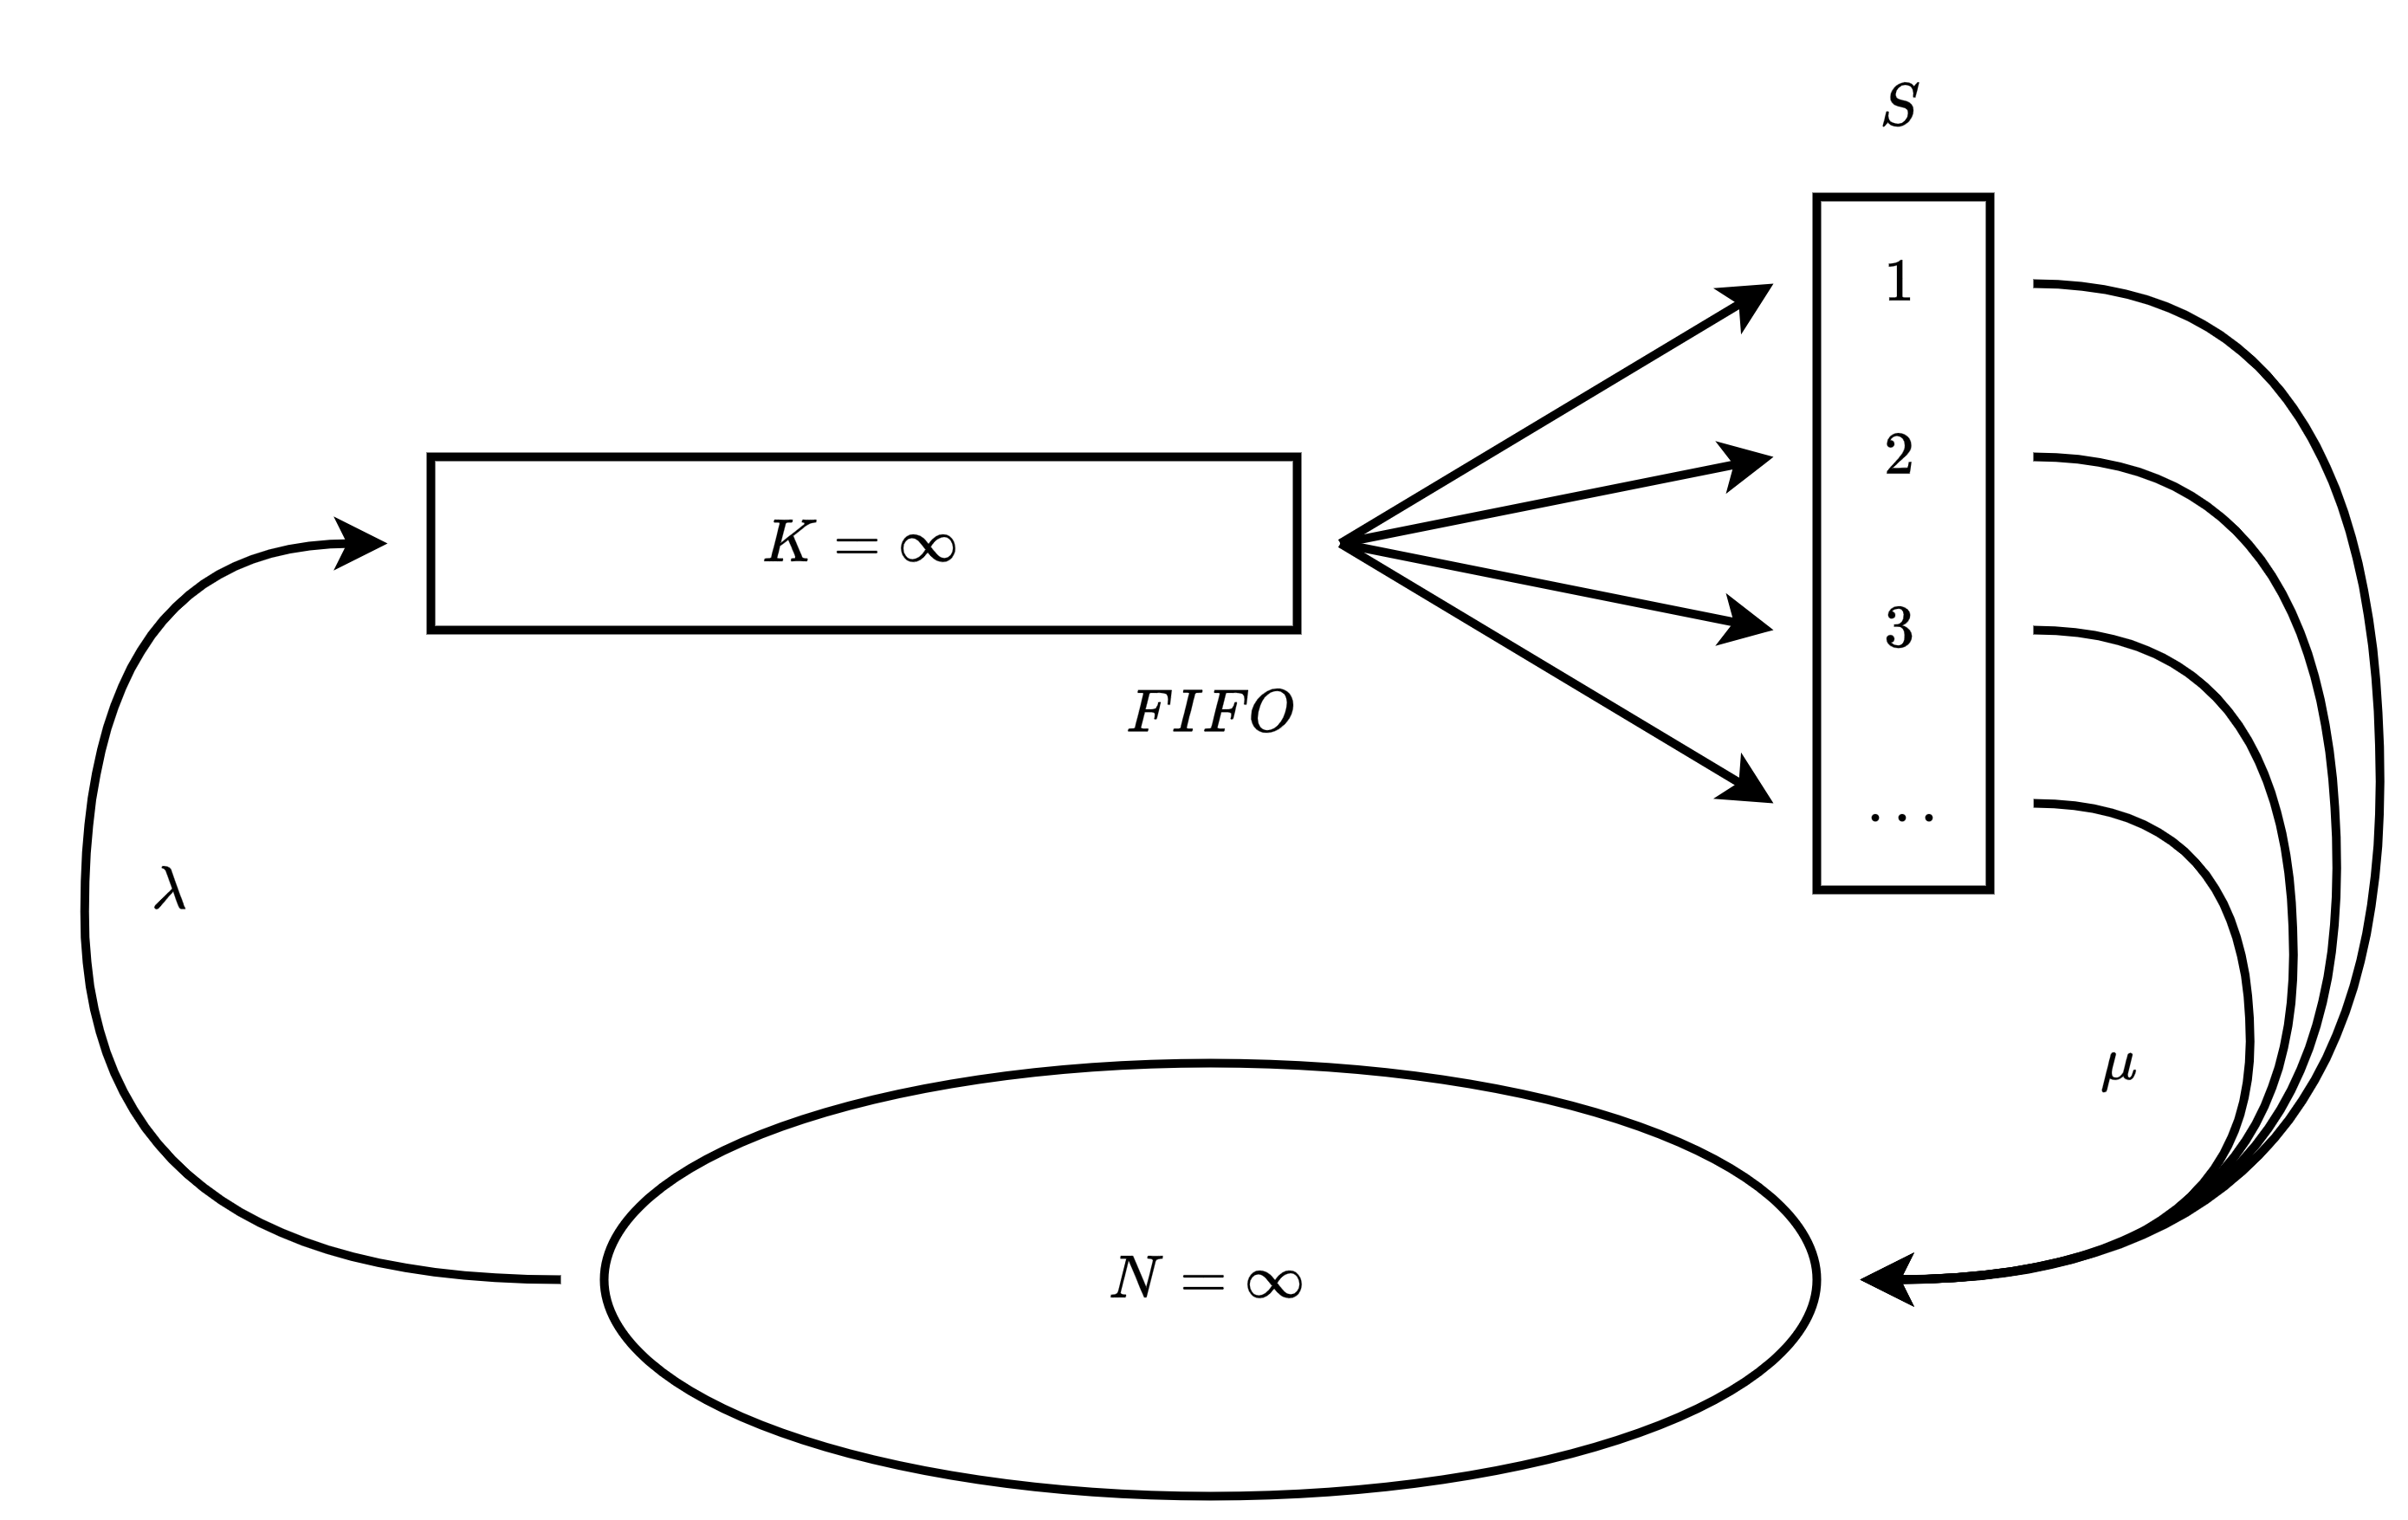
\includegraphics[width=0.8\textwidth]{diagram/mms.png}
\end{center}
Donde:
\begin{itemize}
    \item $K$ : Capacidad del sistema.
    
    \item $S$ : Número de servidores en paralelo.
    
    \item $\mu$ : Tasa de servicio medidas (Clientes / Unidad de tiempo).
    
    \item $N$ : Número de clientes en el sistema.
    
    \item $\lambda$ : Tasa de llegada de clientes (Clientes / Unidad de tiempo)
\end{itemize}

\newpage
\subsection{Indicadores (Performance)}
\textbf{IMPORTANTE:} Para los cálculos, se debe considerar la misma unidad de tiempo.
\begin{itemize}
    \item $L_s$ : Cantidad promedio de clientes en el sistema.
    \begin{equation*}
        L_s = L_q + \frac{\lambda}{\mu} \qquad (L_s = \lambda \cdot W_s)
    \end{equation*}

    \item $L_q$ : Cantidad promedio de clientes en la cola.
    \begin{equation*}
        L_q = \frac{\left(\frac{\lambda}{\mu}\right)^s \cdot \lambda \cdot \mu}{(s-1)! \cdot (s \cdot \mu - \lambda)^2} \cdot P_0 = \frac{1}{s!} \cdot \left(\frac{\lambda}{\mu}\right)^s \cdot \frac{\rho}{(1-\rho)^2} \cdot P_0
    \end{equation*}

    \item $W_s$ : Tiempo promedio de un cliente en el sistema.
    \begin{equation*}
        W_s = W_q + \frac{1}{\mu} \qquad (W_s = \frac{L_s}{\lambda})
    \end{equation*}

    \item $W_q$ : Tiempo promedio de un cliente en la cola.
    \begin{equation*}
        W_q = \frac{L_q}{\lambda} \qquad (L_q = \lambda \cdot W_q)
    \end{equation*}
\end{itemize}

\subsection{Probabilidades}
Sea $n$ : Cantidad de clientes en el sistema. ($n=1,2,...$)
Entonces:
\begin{itemize}
    \item $\rho$ : Factor de utilizaci\'on / Factor de carga / Intensidad tr\'afico.
    \begin{equation*}
        \rho = \frac{\lambda}{s \cdot \mu}
    \end{equation*}

    \item $P_0$ : Probabilidad de que ning\'un cliente se encuentre en el sistema.
    \begin{equation*}
        P_0 = \frac{1}{\displaystyle\sum_{n=0}^{s-1}{\frac{\left(\frac{\lambda}{\mu}\right)^n}{n!} + \frac{\left(\frac{\lambda}{\mu}\right)^s}{s!} \cdot \left(\frac{s \cdot \mu}{s \cdot \mu - \lambda}\right)}}
    \end{equation*}
    
    \item $P_n$ : Probabilidad de que haya $n$ clientes en el sistema.
    \begin{equation*}
        P_n = \begin{cases}
            \displaystyle\frac{\left(\frac{\lambda}{\mu}\right)^n}{n!} \cdot P_0 & \qquad \text{si } n \leq s \\
            \\
            \displaystyle\frac{\left(\frac{\lambda}{\mu}\right)^n}{s! \cdot s^{n-s}} \cdot P_0 & \qquad \text{si } n \geq s
        \end{cases}
    \end{equation*}

    % \item $P(W_q > t)$ : Probabilidad que un cliente este en la cola a lo menos $t$ unidades de tiempo.
    % \begin{equation*}
    %     P(W_q > t) = \rho e^{-\mu(1 - e)\cdot t}
    % \end{equation*}

    % \item $P(W > t)$ : Probabilidad que un cliente permanezca en el sistema, a lo menos $t$ unidades de tiempo.
    % \begin{equation*}
    %     P(W > t) = e^{-\mu(1 - e)\cdot t}
    % \end{equation*}
\end{itemize}

\newpage
\subsubsection{Problema 1:}
Un terminal de facturaci\'on dispone de dos operarios que atienden a los clientes que llegan seg\'un una distribuci\'on de Poisson de media 80 clientes por hora, que esperan en una \'unica cola hasta que alguno de los operarios est\'e libre. El tiempo requerido para atender a un cliente se distribuye exponencialmente con med\'ia 1,2 minutos.
\begin{tcolorbox}[
    colframe=Celeste!100, % Color del borde
    colback=Celeste!20,       % Color del fondo
    coltitle=white!100, % Color del título
    title=\textbf{Datos}, % Título de la caja
]
    $\lambda = 80$ \\
    $W_s = 1,2 \text{ minutos}$ \\
    $\mu = \frac{60}{1,2} = 50$ \\
    $s = 2$ \\
    $\rho = \frac{80}{2 \cdot 50} = \frac{8}{10} < 1 \qquad \text{Condici\'on de regimen}$
\end{tcolorbox}
\begin{enumerate}
    \item ¿Cu\'al es el n\'umero esperado de clientes en el terminal de facturaci\'on?
    \begin{align*}
        L_s &= L_q + \frac{80}{50}
    \end{align*}
    \begin{align*}
        L_q &= \frac{\left(\frac{80}{50}\right)^2 \cdot 80 \cdot 50}{(1)! \cdot (2 \cdot 50 - 80)^2} \cdot P_0
    \end{align*}
    \begin{align*}
        P_0 &= \frac{1}{\displaystyle\sum_{n=0}^{1}{\frac{\left(\frac{80}{50}\right)^n}{n!} + \frac{\left(\frac{80}{50}\right)^2}{2!} \cdot \left(\frac{2 \cdot 50}{2 \cdot 50 - 80}\right)}} \\
        &= \frac{1}{\displaystyle\frac{\left(\frac{80}{50}\right)^0}{0!} + \frac{\left(\frac{80}{50}\right)^1}{1!} + \frac{\left(\frac{8}{5}\right)^2}{2!} \cdot \left(\frac{100}{20}\right)} \\
        &= \frac{1}{1 + \frac{8}{5} + \displaystyle\frac{\frac{64}{25}}{2} \cdot 5} = \frac{1}{1 + \frac{8}{5} + \frac{32}{5}} \\
        &= \frac{1}{1 + \frac{40}{5}} = \frac{1}{1 + 8} = \frac{1}{9} \\
        &= 0,1111
    \end{align*}
    \begin{align*}
        L_q &= \frac{\left(\frac{8}{5}\right)^2 \cdot 80 \cdot 50}{(20)^2} \cdot 0,1111 \\
        &= \frac{\frac{64}{25} \cdot 4000}{400} \cdot 0,1111 = \frac{64}{25} \cdot 10 \cdot 0,1111 \\
        &= 26 \cdot 0,1111 = 2,8886
    \end{align*}
    \begin{align*}
        L_s &= 2,8886 + \frac{80}{50} = 2,8886 + 1,6 \\
        &= 4,4886 \text{ clientes}
    \end{align*}

    \newpage
    \item ¿Cu\'al es el tiempo medio que un cliente pasa en el terminal de facturaci\'on?
    \begin{align*}
        W_s &= \frac{L_s}{\lambda} \\
        &= \frac{4,4886}{80} = 0,0561 \text{ horas} = 3,366 \text{ minutos}
    \end{align*}

    \item Probabilidad de que haya exactamente 6 clientes.
    Como $n > s$:
    \begin{align*}
        P_6 &= \frac{\left(\frac{8}{5}\right)^6}{2! \cdot 2^{6-2}} \cdot 0,1111 \\
        &= \frac{\frac{262144}{15625}}{2^5} \cdot 0,1111 \\
        &= \frac{8192}{15625} \cdot 0,1111 \\
        &= 0,5243 \cdot 0,1111 = 0,0582
    \end{align*}

    \item Probabilidad de que haya menos de 3 clientes.
    \begin{align*}
        P(n < 3) &= P_0 + P_1 + P_2 \\
        &= 0,1111 + \frac{\left(\frac{8}{5}\right)^1}{1!} \cdot 0,1111 + \frac{\left(\frac{8}{5}\right)^2}{2!} \cdot 0,1111 \\
        &= 0,1111 + \frac{8}{5} \cdot 0,1111 + \frac{64}{25} \cdot 0,1111 \\
        &= 0,1111 + 0,1778 + 0,1422 = 0,4311
    \end{align*}
\end{enumerate}

\newpage
\subsubsection{Problema 2:}
Una peque\~na bancaria tiene dos cajeros autom\'aticos que seg\'un una distribuci\'on exponencial atienden a raz\'on de 1,5 minutos por cliente. La tasa de llegada de clientes seg\'un una Poisson es de 30 por hora.
\begin{tcolorbox}[
    colframe=Celeste!100, % Color del borde
    colback=Celeste!20,       % Color del fondo
    coltitle=white!100, % Color del título
    title=\textbf{Datos}, % Título de la caja
]
    $\lambda = 30$ \\
    $W_s = 1,5 \text{ minutos}$ \\
    $\mu = \frac{60}{1,5} = 40$ \\
    $s = 2$ \\
    $\rho = \frac{30}{2 \cdot 40} = \frac{3}{8} < 1 \qquad \text{Condici\'on de regimen}$
\end{tcolorbox}
\begin{enumerate}
    \item N\'umero medio de clientes en el sistema.
    \newline
    \begin{minipage}[t]{0.45\linewidth}
        \begin{align*}
            L_s &= L_q + \frac{30}{40}
        \end{align*}
        \begin{align*}
            L_q &= \frac{\left(\frac{30}{40}\right)^2 \cdot 30 \cdot 40}{(1)! \cdot (2 \cdot 40 - 30)^2} \cdot P_0 \\
            &= \frac{\left(\frac{3}{4}\right)^2 \cdot 30 \cdot 40}{(50)^2} \cdot 0,4545 \\
            &= \frac{\frac{9}{16} \cdot 1200}{2500} \cdot 0,4545 \\
            &= \frac{9}{16} \cdot 0,48 \cdot 0,4545 \\
            &= 0,28125 \cdot 0,4545 \\
            &= 0,1277
        \end{align*}
        \begin{align*}
            L_s &= 0,1277 + \frac{30}{40} = 0,1277 + 0,75 \\
            &= 0,8777 \text{ clientes}
        \end{align*}

    \end{minipage}
    \hfill
    \begin{minipage}[t]{0.45\textwidth}
        \begin{align*}
            P_0 &= \frac{1}{\displaystyle\sum_{n=0}^{1}{\frac{\left(\frac{30}{40}\right)^n}{n!} + \frac{\left(\frac{30}{40}\right)^2}{2!} \cdot \left(\frac{2 \cdot 40}{2 \cdot 40 - 30}\right)}} \\
            &= \frac{1}{\displaystyle\frac{\left(\frac{30}{40}\right)^0}{0!} + \frac{\left(\frac{30}{40}\right)^1}{1!} + \frac{\left(\frac{3}{4}\right)^2}{2!} \cdot \left(\frac{80}{50}\right)} \\
            &= \frac{1}{1 + \frac{3}{4} + \displaystyle\frac{\frac{9}{16}}{2} \cdot 1,6} = \frac{1}{1 + \frac{3}{4} + \frac{9}{20}} \\
            &= \frac{1}{1 + \frac{24}{20}} = \frac{1}{1 + 1,2} = \frac{1}{2,2} \\
            &= 0,4545
        \end{align*}
    \end{minipage}
    

    \item Tiempo medio de un cliente en el sistema.
    \begin{align*}
        W_s &= \frac{L_s}{\lambda} \\
        &= \frac{0,8777}{30} = 0,0293 \text{ horas} = 1,76 \text{ minutos}
    \end{align*}

    \item Porcentaje de tiempo de cajero libre. \newline
    PREGUNTARLE AL PROFESOR.
\end{enumerate}

\newpage
\subsection{\'Unico Servidor con Capacidad Finita (M/M/1/K)}
\noindent
\textbf{Notaci\'on de Kendall:} \hlcolor{Menta}{M}/\hlcolor{Morado!50}{M}/\hlcolor{Turquesa}{1}/\hlcolor{orange}{K} se refiere a un sistema de colas con una \hlcolor{Menta}{tasa de llegada de clientes $\lambda$}, una \hlcolor{Morado!50}{tasa de servicio $\mu$}, \hlcolor{Turquesa}{1 servidor} y una \hlcolor{orange}{cantidad $K$ de clientes en el sistema}.
\newparagraph
\begin{itemize}
    \item Cola finita.
    
    \item El n\'umero m\'aximo de clientes en el sistema es $K$, por lo que la capacidad de la cola es $K-s$.
    
    \item Tiene el formato FIFO (First In First Out).
    
    \item En esta situaci\'on, s\'i el sistema est\'a lleno no se permite la entrada de nuevos clientes al sistema. En consecuencia, la tasa de llegada efectiva no es constante y var\'ia con el tiempo (dependiendo s\'i el sistema est\'a o no lleno).
\end{itemize}
\begin{center}
    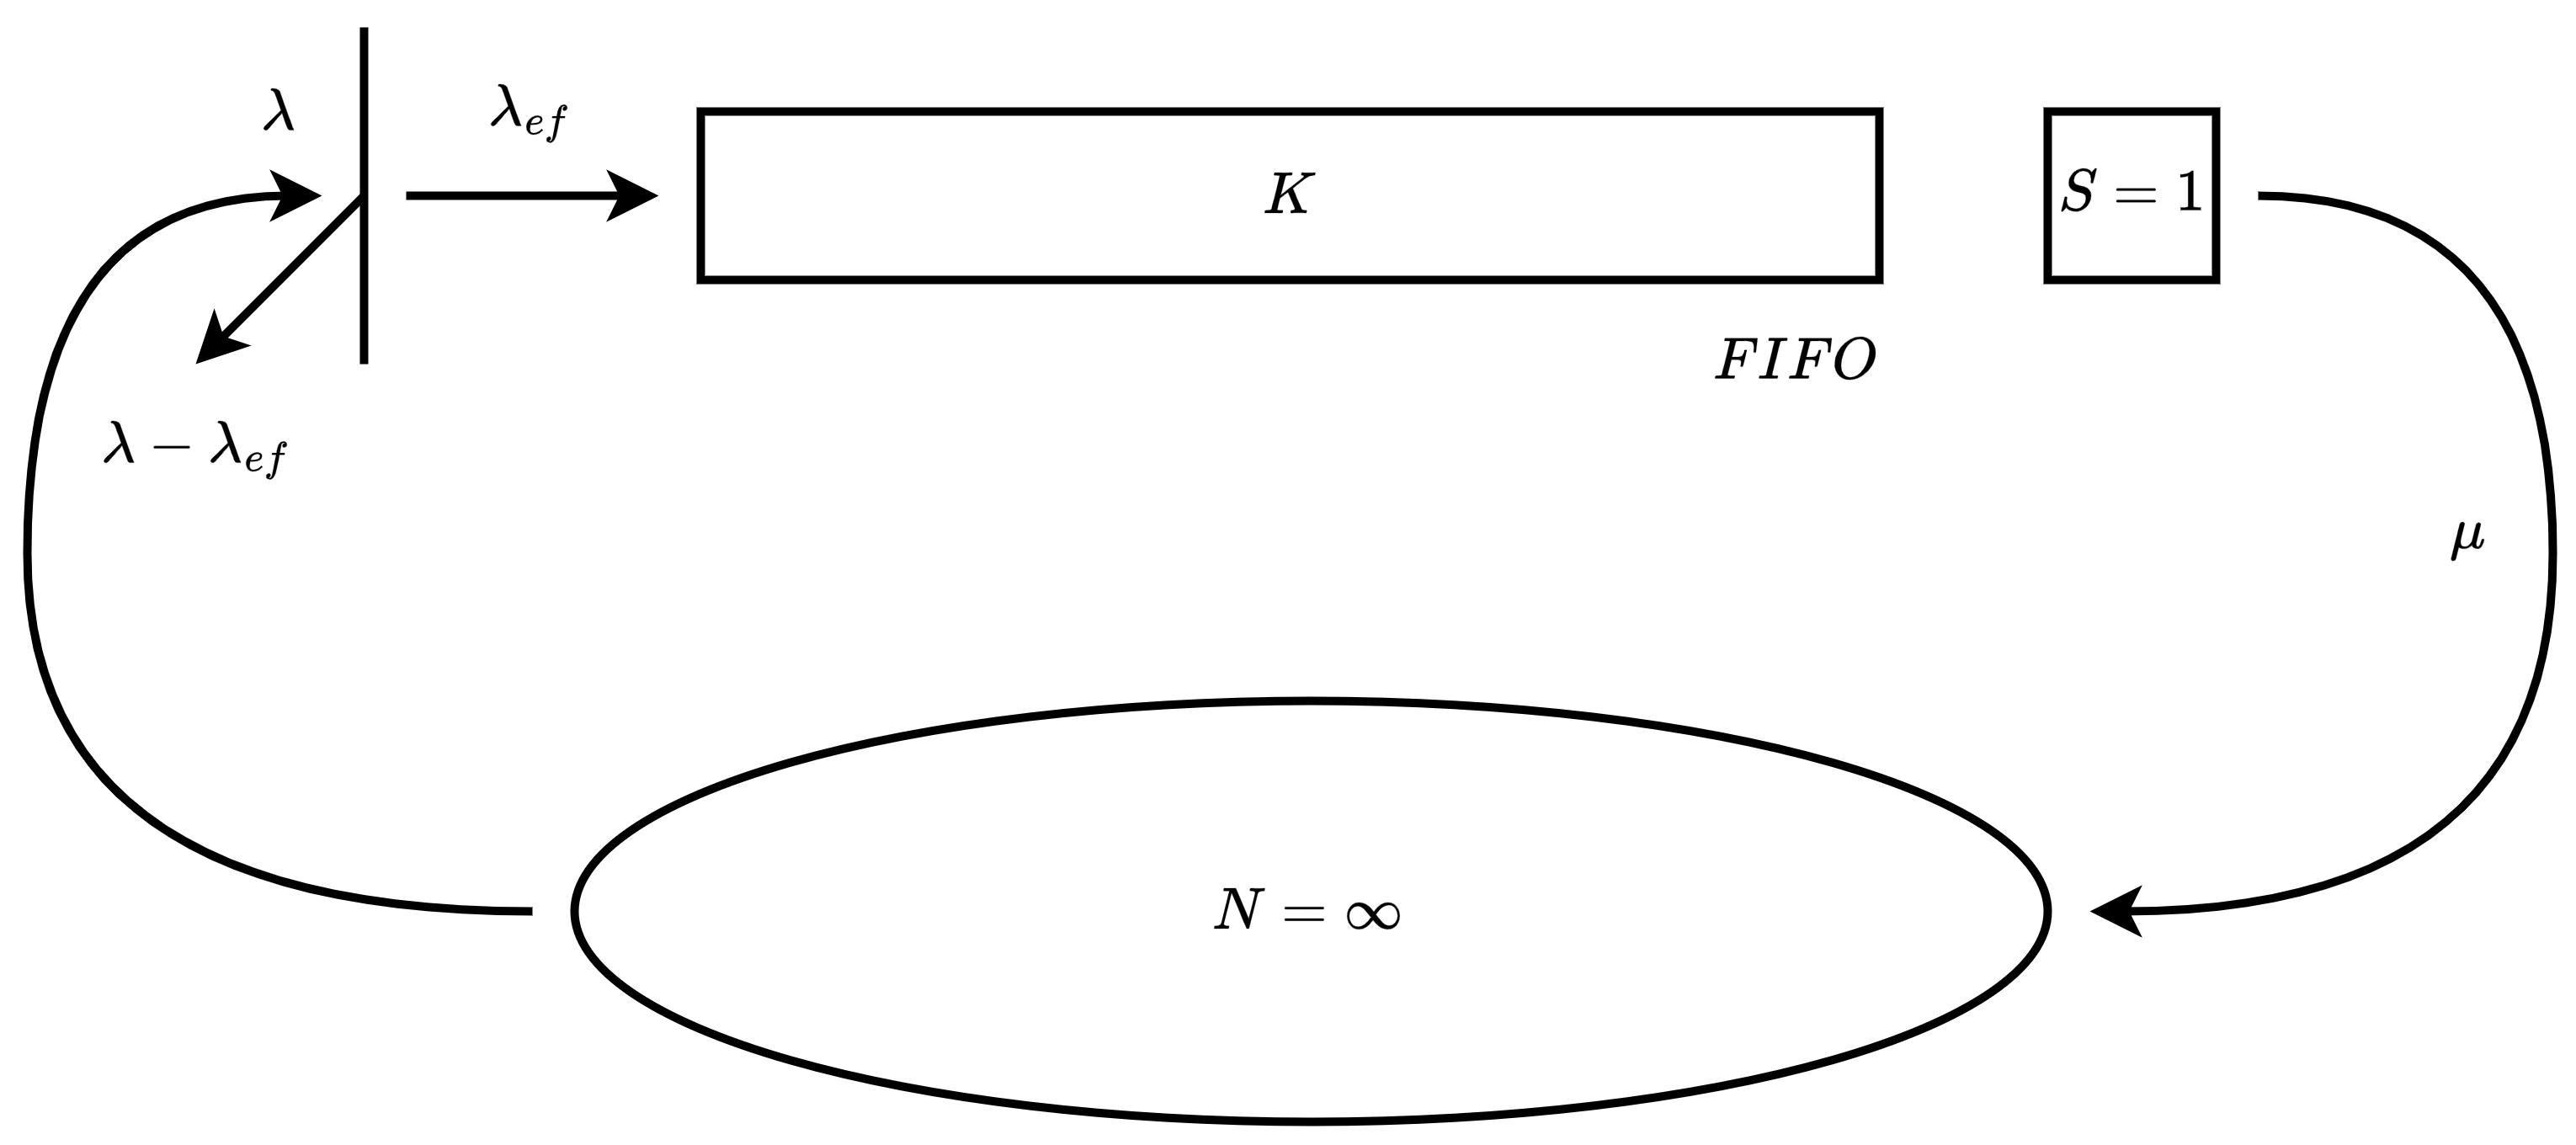
\includegraphics[width=\textwidth]{diagram/mm1k.png}
\end{center}
Donde:
\begin{itemize}
    \item $K$ : Capacidad del sistema.
    
    \item $S$ : Número de servidores en paralelo.
    
    \item $\mu$ : Tasa de servicio medidas (Clientes / Unidad de tiempo).
    
    \item $N$ : Número de clientes en el sistema.
    
    \item $\lambda$ : Tasa de llegada de clientes (Clientes / Unidad de tiempo) 
    
    \item $\lambda_{ef}$ : Tasa de llegada efectiva de clientes.
    \begin{equation*}
        \lambda_{ef} = \lambda \cdot (1 - P_k)
    \end{equation*}
\end{itemize}

\newpage
\subsection{Indicadores (Performance)}
\textbf{IMPORTANTE:} Para los cálculos, se debe considerar la misma unidad de tiempo.
\begin{itemize}
    \item $L_s$ : Cantidad promedio de clientes en el sistema.
    \begin{equation*}
        L_s = \begin{cases}
            \displaystyle\frac{\rho}{(1 - \rho)} - \frac{(k + 1)\cdot \rho^{k+1}}{1 - \rho^{k+1}} & \qquad \text{si } \rho \neq 1 \\
            \\
            \displaystyle\frac{k}{2} & \qquad \text{si } \rho = 1 \\
        \end{cases}
    \end{equation*}

    \item $L_q$ : Cantidad promedio de clientes en la cola.
    \begin{equation*}
        L_q = L_s - (1 - P_0) = \begin{cases}
            \displaystyle L_s - \frac{(1 - \rho^k) \cdot \rho}{1 - \rho^{k + 1}} & \qquad \text{si } \rho \neq 1 \\
            \\
            \displaystyle \frac{k \cdot (k - 1)}{2 \cdot (k + 1)} & \qquad \text{si } \rho = 1 \\
        \end{cases}
    \end{equation*}

    \item $W_s$ : Tiempo promedio de un cliente en el sistema.
    \begin{equation*}
        W_s = \frac{L_s}{\lambda_{ef}}
    \end{equation*}

    \item $W_q$ : Tiempo promedio de un cliente en la cola.
    \begin{equation*}
        W_q = W_s - \frac{1}{\mu} = \frac{L_q}{\lambda_{ef}}
    \end{equation*}


    \item $Long_q$ : Longitud de la cola.
    \begin{equation*}
        Long_q = \lambda_{ef} \cdot W_q
    \end{equation*}
\end{itemize}

\subsection{Probabilidades}
En este sistema da $\rho$ puede tener cualquier valor, pues el sistema no se desborda. \newline
Sea $n$ : Cantidad de clientes en el sistema. ($n=1,2,...$)
Entonces:
\begin{itemize}
    \item $P_0$ : Probabilidad de que ning\'un cliente se encuentre en el sistema.
    \begin{equation*}
        P_0 = \begin{cases}
            \displaystyle \frac{1 - \rho}{1 - \rho^{k + 1}} & \qquad \text{si } \lambda \neq \mu \equiv \rho = \frac{\lambda}{\mu} \neq 1 \\
            \\
            \displaystyle \frac{1}{1 + k} & \qquad \text{si } \lambda = \mu \equiv \rho = \frac{\lambda}{\mu} = 1
        \end{cases}
    \end{equation*}
    
    \item $P_n$ : Probabilidad de que haya $n$ clientes en el sistema.
    \begin{equation*}
        P_n = \begin{cases}
            \displaystyle \rho^n \cdot \frac{(1 - \rho)}{1 - \rho^{k + 1}} & \qquad \text{si } \lambda \neq \mu \equiv \rho = \frac{\lambda}{\mu} \neq 1 \\
            \\
            \displaystyle \frac{1}{1 + k} & \qquad \text{si } \lambda = \mu \equiv \rho = \frac{\lambda}{\mu} = 1
        \end{cases}
    \end{equation*}
\end{itemize}

\newpage
\subsubsection{Problema 1:}
En un taller mec\'anico llegan veh\'iculos para una puesta a punto antes de pasar la ITV, las llegadas siguen un proceso de Poisson de promedio 18 veh\'iculos/hora. Las dimensiones del taller s\'olo permiten que haya 4 veh\'iculos, y las ordenanzas municipales no permiten esperar en la v\'ia p\'ublica. El taller despacha un promedio de 6 veh\'iculos/hora de acuerdo con una distribuci\'on exponencial. Se pide:
\begin{enumerate}
    \item ¿Cu\'al es la probabilidad de uqe no haya ning\'un veh\'iculo en el taller?
    
    \item ¿Cu\'al es el promedio de veh\'iculos en el taller?
    
    \item ¿Cu\'anto tiempo pasa por t\'ermino medio un veh\'iculo en el taller?
    
    \item ¿Cu\'anto tiempo esperan por t\'ermino medio los veh\'iculos en la cola?
    
    \item ¿Cu\'al es la longitud media de la cola?
\end{enumerate}
\newpage
\subsubsection{Problema 2:}
Sea un sistema de espera (m/m/1/6) y $\lambda = \mu = 20$.
Calcular:
\begin{enumerate}
    \item $L_s$.
    \begin{align*}
        L_s &= \frac{k}{2} \\
        &= \frac{6}{2} \\
        &= 3
    \end{align*}

    \item $L_q$.
    \begin{align*}
        L_q &= \frac{k \cdot (k - 1)}{2 \cdot (k + 1)} \\
        &= \frac{6 \cdot 5}{2 \cdot 7} \\
        &= 2,1429
    \end{align*}

    \item Probabilidad de que hayan menos de 3 clientes en el sistema.
    \begin{align*}
        P(n > 3) &= P_0 + P_1 + P_2 \\
        &= \frac{1}{7} + \frac{1}{7} + \frac{1}{7} = \frac{3}{7} \\
        &= 0,4286
    \end{align*}

    \item Tasa efectiva.
    \begin{align*}
        \lambda_{ef} &= \lambda \cdot (1 - P_0) \\
        &= 20 \cdot (1 - \frac{1}{7}) \\
        &= 20 \cdot (\frac{6}{7}) \\
        &= \frac{120}{7} \\
        &= 17.1429
    \end{align*}

    \begin{figure}[H]
        \centering
        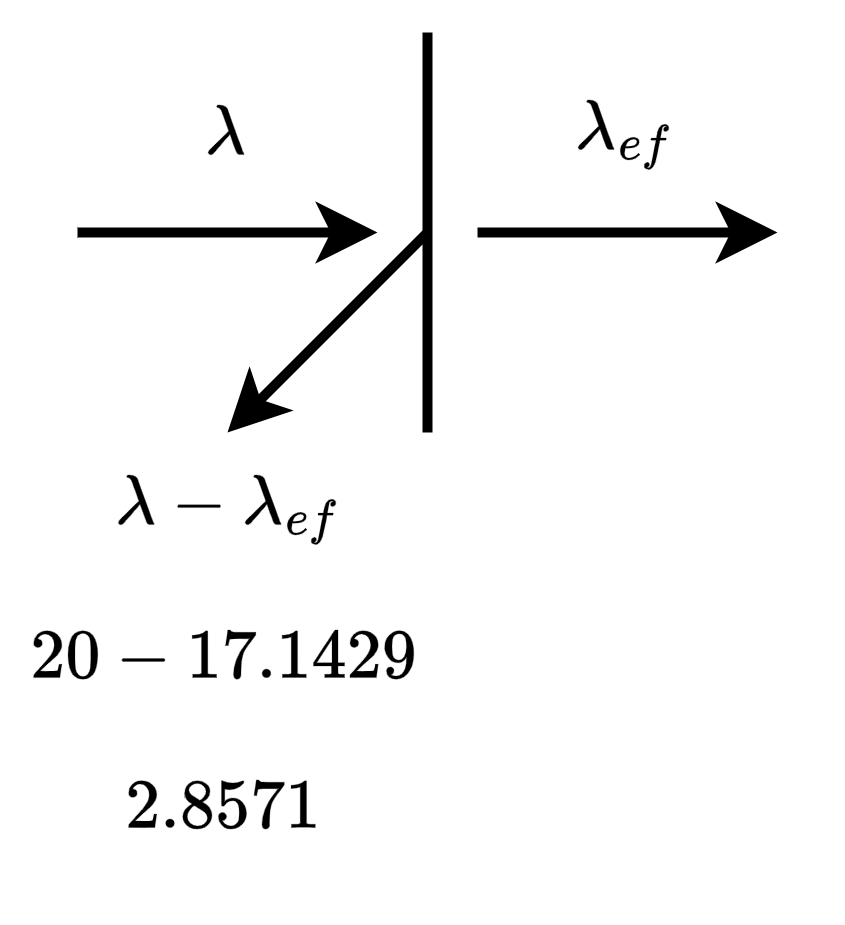
\includegraphics[width=0.3\textwidth]{diagram/tasaefectiva.png}
    \end{figure}
\end{enumerate}
\newpage
\section{Costos en los sistemas de colas}
\begin{equation*}
    C_t = S \cdot C_s + L \cdot C_w
\end{equation*}
\begin{center}
    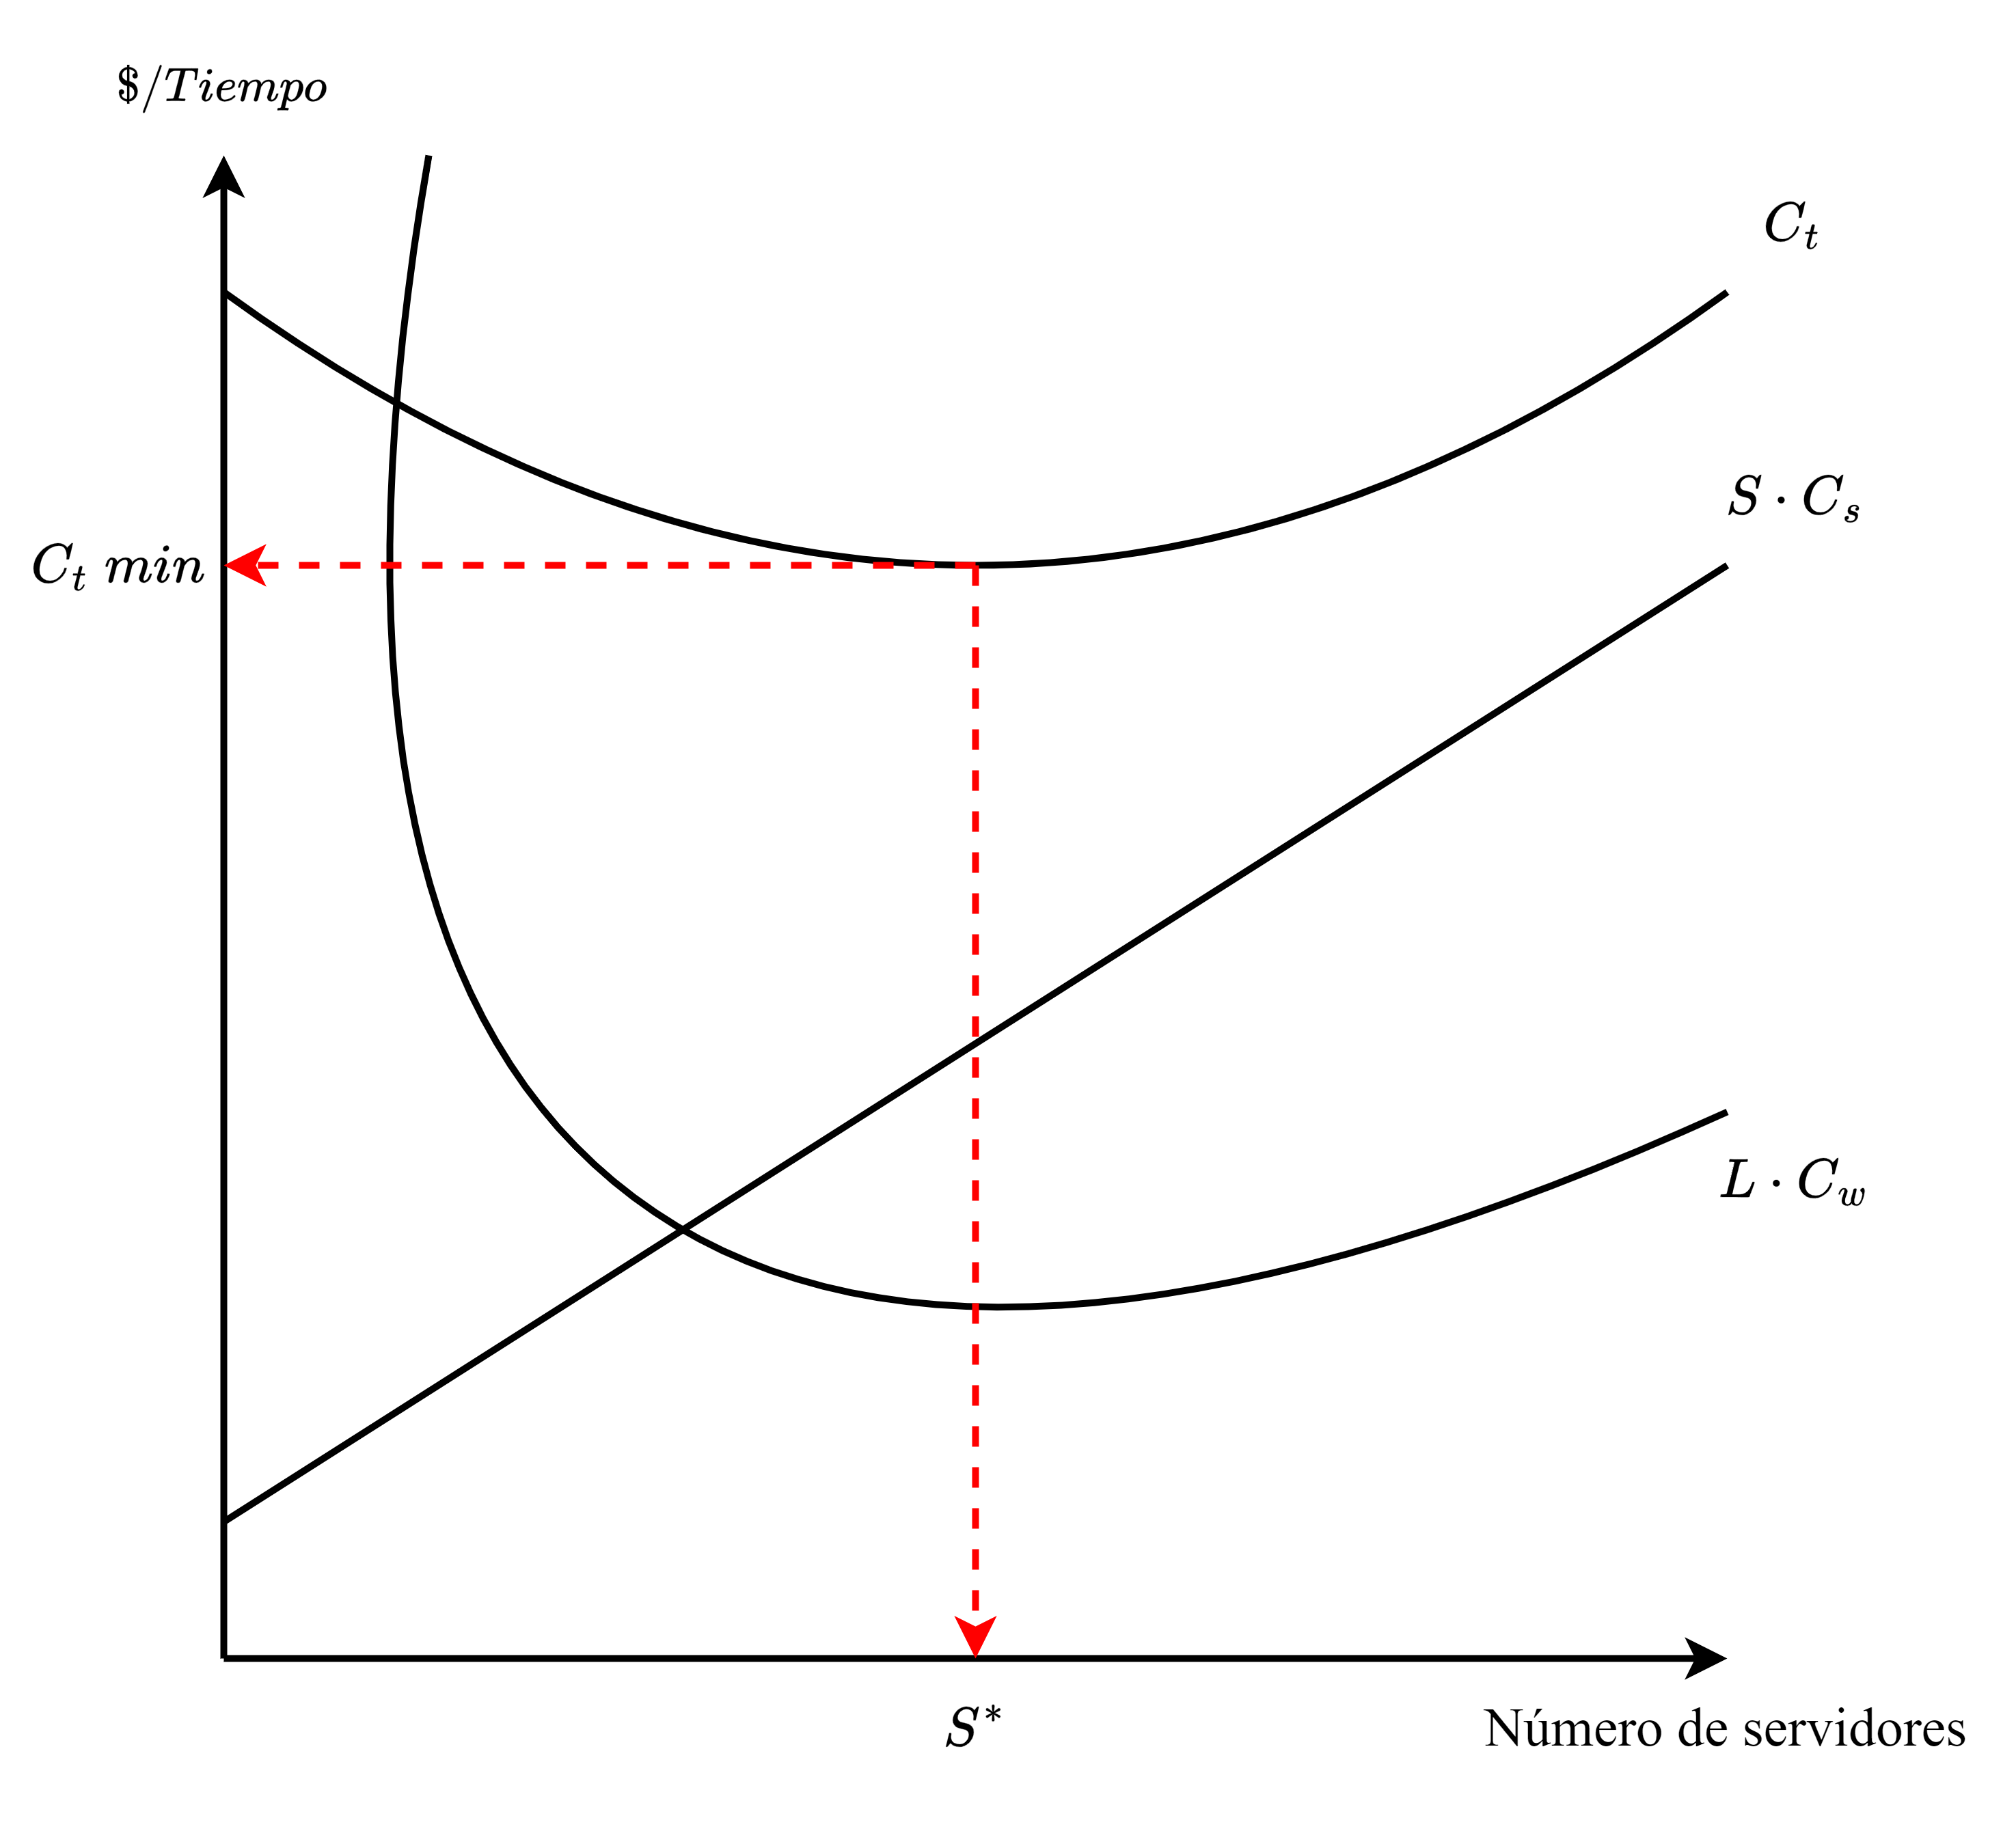
\includegraphics[width=0.8\textwidth]{diagram/Costos.png}
\end{center}
Donde:
\begin{itemize}
    \item $S$ : N\'umero de servidores.
    
    \item $C_s$ : Costo de operaci\'on por servidor (\$/t).
    
    \item $L$ : N\'umero promedio de clientes.
    
    \item $C_w$ : Costo unitario de espera (\$/t).
\end{itemize}

\newpage
\subsection{Problema 1:}
El departamento de Ciencias de la Decisi\'on trata de determinar si renta una copiadora lenta o una r\'apida. El departamento cree que el tiempo de un empleado vale 15 \$/h. El arrendamiento de la copiadora lenta cuesta 4 \$/h y un empleado tarda un promedio de 10 minutos en terminar sus copias, distribuido exponencialmente. La copiadora r\'apida cuesta 15 \$/h en arrendamiento, y un empleado tarda un promedio de 6 minutos en terminar sus copias. Un promedio de 4 empleados/h son los que necesitan usar la copiadora. Los tiempos entre llegadas son exponenciales. ¿Que maquina debe rentar el departamento?
\begin{center}
    \begin{tabular}{|c|c|c|}
        \hline
        & m/m/1 lenta & m/m/1 r\'apida \\ \hline
        $s$ & 1 & 1 \\ \hline
        $C_s$ & 4 \$/h & 15 \$/h \\ \hline
        $\lambda$ & 4 empleados/h & 4 empleados/h \\ \hline
        $\mu$ & 6 clientes/h & 10 clientes/h \\ \hline
        &&\\
        $L$ & $\displaystyle\frac{4}{2} = 2$ & $\displaystyle\frac{4}{6} = \frac{2}{3}$ \\
        &&\\ \hline
        $C_w$ & 15 \$/h & 15 \$/h \\ \hline
        &&\\
        $C_t$ & $1 \cdot 4 + 2 \cdot 15 = 34$ \$/h & $1 \cdot 15 + \displaystyle\frac{2}{3} \cdot 15 = 25$ \$/h \\
        &&\\ \hline
    \end{tabular}
\end{center}
\begin{equation*}
    \therefore \text{Se debe arrendar la fotocopiadora r\'apida.}
\end{equation*}

\subsection{Problema 2:}
Un supermercado trata de decidir cu\'antas cajas deben estar funcionando. Suponga que cada hora llega un promedio de 18 clientes, y el tiempo promedio de atenci\'on a un cliente es 4 minutos. Los tiempos entre llegadas y los tiempos de servicio son exponenciales, y el sistema se puede modelar como uno $M/M/s/DG/\infty/\infty$. El funcionamiento de una caja cuesta 20 \$/h, y se carga un costo de 0,25 \$ por cada minuto que el cliente pasa en la zona de cajas. ¿Cu\'antas cajas debe abrir el supermercado?
\begin{center}
    \begin{tabular}{|c|c|c|}
        \hline
        $s$ & $P_0$ & $L$ \\ \hline
        1 & - & - \\
        2 & 0,25 & 1,88 \\
        3 & 0,29 & 1,29 \\
        4 & 0,3 & 1,22 \\ \hline
    \end{tabular}
\end{center}
\begin{center}
    \begin{tabular}{ccccccc|l}
        $s$ & $\mu$ & $\lambda$ & $\rho$ & $C_s$ & $L$ & $C_w$ & $C_t$\\ \hline
        1 & 15 & 18 & Colapsa & 20 & - & 15 & - \\
        2 & 15 & 18 & Estable & 20 & 1,88 & 15 & $40 + 1.88 \cdot 15 = 68.2$* \\
        3 & 15 & 18 & Estable & 20 & 1,29 & 15 & $60 + 1.29 \cdot 15 = 79.35$ \\
        4 & 15 & 18 & Estable & 20 & 1,22 & 15 & $80 + 1.22 \cdot 15 = 98.3$ \\
        ... & ... & ... & ... & ... & ... & ... & ... \\
    \end{tabular}
\end{center}
\end{document}